\chapter{Implementation}
In this chapter, I will explain in detail, how the different parts of the project were designed and built.

%%%%%%%%%%%%%%%%%%%%%%%%%%%%%%%%%%%%%%%%%%%%%%%%%%%%%%%%%%%%%%%%%%%%%%%%%%%%
%% explain the data models
%%
%%%%%%%%%%%%%%%%%%%%%%%%%%%%%%%%%%%%%%%%%%%%%%%%%%%%%%%%%%%%%%%%%%%%%%%%%%%%
\section{Data Models}

The system needs to handle data regarding - 

\begin{itemize}
	\item \textit{People} who will use the system.
	\item Details of \textit{Something} that can be traded, lent, rented or sold etc.
	\item Record of \textit{interaction} between people regarding some item of interest.	
\end{itemize}

Data models were designed keeping these in mind. The models were developed as they were needed for user stories during a sprint.

%%%%%%%%%%%%%%%%%%%%%%%%%%%
%% Model defs
%%
%%%%%%%%%%%%%%%%%%%%%%%%%%%
\subsection{Model Definitions}

\begin{description}
	\item [User] : Users must have a unique username and a password (hashed). They can also have a default avatar (as Base64 or URI) and an initial rating of 0. Rating is primitive and only accounts for the average.
	\item [PushToken] : Every User must have a PushToken object reference. These objects contain the device tokens generated by GCM by push registration.
\end{description}

%% user data model diagram
\begin{figure}[!h]
\centering
\begin{tikzpicture}

\umlclass[x=0, y=0]{User}{
  \textbf{* username} : \texttt{String} \\
  \textbf{* password} : \texttt{String}\\
  \textbf{\_pushTokens} : \texttt{PushToken.\_id}\\
  \textbf{avatar} : \texttt{String}\\
  \textbf{rating} : \texttt{\{ count : Number, average: Number \}}\\
}{}

\umlclass[x=8, y=0]{PushToken}{
  \textbf{* \_user} : \texttt{User.\_id} \\
  \textbf{tokens} : \texttt{[String]}\\
}{}

\end{tikzpicture}
\caption{User Model} \label{fig:user-model}
\end{figure}

\begin{description}
	\item [Thing] : A Thing is an abstraction for either a service or an object. It must have a name and an owner. Other fields include name, description and type (category). \texttt{closed} records whether the item can be acquired or not, whereas \texttt{\_reservedTo} is the User whose offer for the thing was last accepted.
	\item [Lend] : A Lend object is created when a User wants others to borrow a Thing (which gets a reference to that object).
\end{description}

%% Thing data model diagram
\begin{figure}[!h]
\centering
\begin{tikzpicture}

\umlclass[x=0, y=0]{Thing}{
  \textbf{* name} : \texttt{String} \\
  \textbf{type} : \texttt{String}, \\
  \textbf{desc}: \texttt{String}, \\
  \textbf{* \_owner} : \texttt{User.\_id}\\
  \textbf{pictures} : \texttt{[String]}\\
  \textbf{\_lend} : \texttt{Lend.\_id}\\
  \textbf{\_sell} : \texttt{Sell.\_id}\\
  \textbf{\_reservedTo} : \texttt{Offer.\_id}\\
  \textbf{closed} : \texttt{Boolean}\\
}{}

\umlclass[x=6, y=0.5]{Offer}{
  \textbf{* \_from} : \texttt{User.\_id} \\
  \textbf{* \_to} : \texttt{User.\_id}, \\
  \textbf{* \_borrow}: \texttt{Lend.\_id}, \\
  \textbf{* \_buy} : \texttt{Sell.\_id}\\
  \textbf{reason} : \texttt{String}\\
  \textbf{accepted} : \texttt{Boolean}\\
  \textbf{declined} : \texttt{Boolean}
}{}

\umlclass[x=0, y=-5]{Sell}{
  \textbf{* \_thing} : \texttt{Thing.\_id} \\
  \textbf{price} : \texttt{Number}
}{}

\umlclass[x=6, y=-4.5]{Lend}{
  \textbf{* \_thing} : \texttt{Thing.\_id} \\
  \textbf{deposit} : \texttt{Number}, \\
  \textbf{from}: \texttt{Date}, \\
  \textbf{to} : \texttt{Date}\\
}{}

\end{tikzpicture}
\caption{Thing Model} \label{fig:thing-model}
\end{figure}

\begin{description}
	\item [Sell] : Similar to Lend, it only gets created when a User wants others to buy a Thing. A Thing can have both \texttt{\_sell} and \texttt{\_lend}.
	\item [Offer] : An Offer is created when a User wants to buy/borrow (depending on which options are available) some item for some \textit{reason}. It can be accepted or declined (both initially set to false).
\end{description}

\subsection{Model Design Choices}

Things can be \textit{closed}, rather than removed from the system once a transaction takes place, so that, a borrowed item could be made \textit{active} once it has been returned, rather than posting again.\\

Offers have both \textit{accepted} and \textit{declined} fields, rather than a toggle, because, the initial condition, where it is neither accepted nor declined, can be interpreted.\\

Images, as explained in Section \ref{subsec:issues}, are saved directly as Strings, rather than BLOBs (Binary Large OBject) because of database free account restriction.\\

User objects do not directly have access to device tokens, so that, unused or invalid tokens can be destroyed in future without manipulating the main User object.\\

Lend or Sell options are whole objects, rather than a field on a Thing, because, an Offer should be distinguished between a borrow or a buy offer. Rather than creating an Offer hierarchy, these intermediate objects are referenced in respective Offer-Thing combos.

\section{Server}

In this section, I will discuss how the RESTful API was created, database and GCM integration was done and how authentication is performed.

\subsection{Routes}

\href{https://en.wikipedia.org/wiki/Representational_state_transfer}{REST} (Representational State Transfer) is the software architectural style of WWW (World Wide Web) \cite{Fielding:2000}. Simply put, a client makes requests, usually HTTP (Hypertext Transfer Protocol) requests, at specific routes. The methods are usually CRUD (Create Read Update Delete).\\

This server was then hosted on heroku at \href{http://project-api.herokuapp.com/}{http://project-api.herokuapp.com/}. Each route is superseded by \texttt{/api} to denote a version number for the api. Table \ref{table:user-routes}, \ref{table:thing-routes} and \ref{table:offers-routes} respectively shows routes for User, Thing and Offer objects. These routes were created with the following in mind -

\begin{itemize}
	\item Users will need to add new items, retrieve all or searched items.
	\item The things will be updated, requested upon and eventually closed.
	\item Users will want to request for items, respond to requests and rate others.
\end{itemize}

\newcommand{\NA}{---}

\begin{table}[!h]
    \centering
    \begin{tabularx}{\textwidth}{lcXcc}
    \toprule
    \centering
    \emph{\textbf{Route}} \texttt{/users} & \emph{\textbf{Method}} & \emph{\textbf{Use}} & \emph{\textbf{Params}} & \emph{\textbf{Returns}} \\
    \midrule
    \texttt{/}
    		& \texttt{GET} & get all the \newline users on the system  & \NA 			 & \texttt{[User]} \\ \cline{2-5} \noalign{\smallskip}
    		& \texttt{POST} & create a new user on the system  & \texttt{User}  & \texttt{User}    \\ 
    \midrule
    \texttt{/:uname} 
    		& \texttt{GET} & get a particular user & \NA & \texttt{User}  \\ \cline{2-5} \noalign{\smallskip}
    		& \texttt{PUT} & update a single user & \texttt{User} & \texttt{User} \\
    	\midrule
    \texttt{/:uname/things}
    		& \texttt{GET} & get all the things for a user & \NA & \texttt{[Thing]} \\ \cline{1-5} \noalign{\smallskip}
    \texttt{/:uname/rating}
    		& \texttt{PUT} & rate a user & \texttt{[User.rating]} & \NA  \\ \cline{1-5} \noalign{\smallskip}
	\texttt{/offers/to}
		& \texttt{GET} & get all the offers made to a user & \NA & \texttt{[Offer]}  \\
    \bottomrule
    \hline
    \end{tabularx}
    \caption{User Routes}
    \label{table:user-routes}
\end{table}

\begin{table}[!h]
    \centering
    \begin{tabularx}{\textwidth}{lcXcc}
    \toprule
    \centering
    \emph{\textbf{Route}} & & & \\
    \texttt{/things} & \emph{\textbf{Method}} & \emph{\textbf{Use}} & \emph{\textbf{Params}} & \emph{\textbf{Returns}} \\
    \midrule
    \texttt{/}
    		& \texttt{GET} & get all the things on system  & \NA 			& \texttt{[Thing]} \\ \cline{2-5} \noalign{\smallskip}
    		& \texttt{POST} & create a new thing on system & \texttt{Thing} & \texttt{Thing} \\
	\midrule    	
    	\texttt{/:id}
    		& \texttt{GET} & get a particular thing & \NA & \texttt{Thing} \\ \cline{2-5} \noalign{\smallskip}
    		& \texttt{PUT} & update a single thing & \texttt{Thing} & \texttt{Thing} \\ \cline{2-5} \noalign{\smallskip}
    		& \texttt{DELETE} & delete a single thing & \NA & \texttt{Thing} \\
    	\midrule
    	\texttt{/:id/close}
    		& \texttt{POST} & close a single thing & \NA & \texttt{Thing} \\
    \bottomrule
    \hline
    \end{tabularx}
    \caption{Thing Routes}
    \label{table:thing-routes}
\end{table}

\begin{table}[!h]
    \centering
    \begin{tabularx}{\textwidth}{lcXcc}
    \toprule
    \centering
    \emph{\textbf{Route}} & & & \\
    \texttt{/things/:id/offers} & \emph{\textbf{Method}} & \emph{\textbf{Use}} & \emph{\textbf{Params}} & \emph{\textbf{Returns}}\\
    \midrule
    \texttt{/:offer\_id}
    		& \texttt{GET} & get all offers for a thing & \NA & \texttt{[Thing]} \\ \cline{1-5} \noalign{\smallskip}
    	\texttt{/:offer\_id/accept}
    		& \texttt{GET} & accept an offer & \NA & \texttt{Thing} \\ \cline{1-5} \noalign{\smallskip}
    	\texttt{/:offer\_id/decline}
    		& \texttt{POST} & decline an offer & \NA & \texttt{Thing} \\
    \bottomrule
    \hline
    \end{tabularx}
    \caption{Offers Routes}
    \label{table:offers-routes}
\end{table}

\subsection{Code Structure}

There are 3 main sections in this server :

\begin{description}
	\item [Models] is where the \texttt{mongoose} data models are defined. Any data field validation, pre-post hooks to methods (e.g. a \textit{post} hook to \textit{delete} a User object deletes the corresponding \textit{PushToken} object from DB) etc. are done here.
	\item [Controllers] is where the callbacks for the http request handling are defined. Specially, \texttt{rest-framework.js} file contains my own simple framework to support HTTP GET, POST, PUT \& DELETE methods. There is a controller for each model that is directly accessed from the client app.
	\item [Server] is where the server configurations and http routes are defined. \texttt{server.js} attaches methods from the controllers to respective routes, e.g. \texttt{ThingController.postThings} is attached to \texttt{/things} route.
\end{description}

\subsection{Authentication using Passport}

\href{http://passportjs.org}{Passport} is a NodeJS module which provides different strategies to authenticate applications including various social networks. In this project, I used the \textit{Basic Strategy} or \textit{BasicAuth} for authentication. Which means, each User object has a password that is hashed using \textit{bcrypt} before it is saved to the database. A \texttt{passport.js} strategy is defined in \texttt{authController.js} which verifies a provided \textit{plain text} password against the hashed password on the database. This strategy is then used to intercept every connection (except to create a new User), authenticate said connection and finally serve it. A failure to authenticate results in a HTTP 401 error.

\subsection{Database Integration}

\href{http://mongoosejs.com}{Mongoose} is a NodeJS module which provides built in type casting, validation, query building, hooks etc. for a MongoDB database. A database was created using a free service on mLab and an admin user was added. This admin, along with the database address was then put in configuration in \texttt{server.js}, thus establishing the connection. Mongoose provides an easy to understand \textit{schema-like} definition structure to a NoSQL database. Mongoose also adds timestamps for object creation (\texttt{createdAt}) and latest update (\texttt{updatedAt}) to the object. It also provides an optional  \texttt{populate} method to add all the referenced objects, when an object is retrieved.

\subsection{GCM Integration}

GCM is integrated in the server using the \href{https://www.npmjs.com/package/node-gcm}{node-gcm} module. First, I created a new project on GAE(Google App Engine), then added a server key for a GCM API. This key was then put in the configuration. At this point a notification request can be sent to GCM, given an array of device tokens and other parameters (e.g. the title, body, sound, icon etc.). GCM can be queried for the acceptance of the request, but the actual sending is performed by GCM itself. The messages can have a time-to-live of 3 months, and can arrive at any point in between because only a \textit{free} account is being used.

\section{Client}

\subsection{Ionic Project Structure}

An Ionic project, itself, is a NodeJS module. The \texttt{www/} directory must contain all the \textit{code} using HTML, CSS and JavaScript. \texttt{www/index.html} is the starting point of the app. \texttt{plugins/} is where all the platform specific (e.g. written in Java for Android) plugins are kept. \texttt{platforms/} keeps generated code for different platforms. \texttt{ionic serve -l} will start a local server where both iOS and Android versions of the app are emulated (except for the plugins which are only activated on a mobile).

\subsection{App Structure}

\texttt{ui-router}, an Angular library, is used by Ionic to define the app in forms of \textit{States}. Each state gets a \textit{template} (an HTML file) as view and a \textit{controller} (an AngularJS file) as the view's Angular controller. The controllers share data between themselves using Angular Factories. The template files are kept in \texttt{www/templates/} and all the JavaScript code is in \texttt{www/js/}. Figure \ref{fig:client-app} is a complete representation of the different components in the Client App.

\subsection{States}

Each state gets an URI (e.g. \texttt{/app/profile}). The URI routes to the template view of the app. States can be abstract (e.g. \texttt{app}), with child states (e.g \texttt{app.products}). Data from the database is requested and resolved by the state and injected into the controller before the views are loaded, for example: latest 20 products are fetched on loading the Products state. \texttt{ui-router} also automatically keeps track of navigation by using the states.

\subsection{Controllers}

Controllers hold the various data and functions that are shown or used on the view. For example: using the \texttt{ng-model} directive on a text-box, it can be bound to a variable in the view's controller. Thereafter, any changes to either the textbox or the variable will reflect on the other end. This is achieved by a regular \textit{digest} cycle performed by the Angular engine. However, using many such directives in a view can lead to \textit{significant} performance decrease.

\subsection{Services}

Controllers are view specific. However, there are common tasks that even distinctly different controllers will need to perform, database query for example. These are defined in Angular \textit{Factories} or \textit{Services}. These can be injected in the controllers or the state definitions, but are inaccessible from the view. If a function is needed on the view, it is defined in the controllers and those will, in turn, optionally use services.

%%%%%%%%%%%%%%%%%%%%%%%%%%%%%%
%% The client app diagram
%%
%%%%%%%%%%

\definecolor{amber}{rgb}{1.0, 0.49, 0.0}
\definecolor{applegreen}{rgb}{0.55, 0.71, 0.0}
\definecolor{goldenpoppy}{rgb}{0.99, 0.90, 0.0}
\definecolor{lilac}{rgb}{0.78, 0.64, 0.78}
\definecolor{peridot}{rgb}{0.9, 0.89, 0.0}

\begin{figure}[!h]
\centering
\begin{tikzpicture}

%%%%%%%%%%%%%%%%%%%%%%
%% the app
\begin{umlstate}[name=app]{\textbf{APP}}

%%%%%%%%%%%%%%
%% services
\begin{umlstate}[y = 11, name=services, fill=amber!20]{\textbf{SERVICES}}
\umlbasicstate[name=routeFactory, fill=lilac!20]{\texttt{RouteFactory}}
\umlbasicstate[y = -2.4, name=profileFactory, fill=lilac!20]{\texttt{ProfileFactory}}
\umlbasicstate[y = -4.8, name=loginFactory, fill=lilac!20]{\texttt{LoginFactory}}
\umlbasicstate[y = -7.1, name=productFactory, fill=lilac!20]{\texttt{ProductFactory}}
\end{umlstate}

%%%%%%%%%%%%%%
%% controllers
\begin{umlstate}[x = 5, y = 11, name=controllers, fill=applegreen!20]{\textbf{CONTROLLERS}}
\umlbasicstate[name=appCtrl, fill=peridot!20]{\texttt{AppCtrl}}
\umlbasicstate[y = -2.3, name=productListCtrl, fill=peridot!20]{\texttt{ProductListCtrl}}
\umlbasicstate[y = -4.7, name=categoryCtrl, fill=peridot!20]{\texttt{CategoryCtrl}}
\umlbasicstate[x = 4, name=loginCtrl, fill=peridot!20]{\texttt{LoginCtrl}}
\umlbasicstate[x = 4, y = -2.3, name=productCtrl, fill=peridot!20]{\texttt{ProductCtrl}}
\umlbasicstate[x = 4, y = -4.7, name=profileCtrl, fill=peridot!20]{\texttt{ProfileCtrl}}
\umlbasicstate[x = 2, y = -7, name=notificationCtrl, fill=peridot!20]{\texttt{NotificationCtrl}}
\end{umlstate}

%%%%%%%%%%%%%%%
%% the states bit
\begin{umlstate}[name=states, fill=goldenpoppy!20]{\textbf{STATES}}
\umlbasicstate[x = 4.8, name=menu, fill=red!20]{\texttt{Menu}}
\umlbasicstate[y = -3, name=productList, fill=blue!20]{\texttt{ProductList}}
\umlbasicstate[x = 3.5, y=-3, name=categories, fill=blue!20]{\texttt{Categories}}
\umlbasicstate[x = 6.5, y=-3, name=profile, fill=blue!20]{\texttt{Profile}}
\umlbasicstate[x = 9.4, y=-3, name=requests, fill=blue!20]{\texttt{Requests}}
\umlbasicstate[x = 4.8, y=-6, name=product, fill=blue!20]{\texttt{Product}}
\umlbasicstate[y=-6, name=newProd, fill=blue!20]{\texttt{NewProduct}}
\umltrans{menu}{productList}
\umltrans{menu}{categories}
\umltrans{menu}{profile}
\umltrans{menu}{requests}
\umltrans{productList}{product}
\umltrans{productList}{newProd}
\umltrans{profile}{product}
\umltrans{categories}{product}
\umlbasicstate[x= 8, name=login, fill=green!20]{\texttt{Login}}
\umltrans{login}{menu}
\end{umlstate}

\end{umlstate}

\end{tikzpicture}
\caption{Client App Structure}\label{fig:client-app}
\end{figure}